\section{Auswertung}
\label{sec:Auswertung}

\subsection{Bestimmung des Nulleffekts}\label{sec:Nulleffekt}
Zur Bestimmung des Nulleffekts wurden die Ausschläge des Geiger-Müller-Zählrohrs in einem 
Zeitintervall von $\SI{500}{s}$ gemessen.
Die Messung ergab eine Nulleffektrate von
\begin{equation*}
  N_{0} = \SI{100}{\frac{Impulse}{500s}}.
\end{equation*}

\subsection{Zerfallskurve und Halbwertszeit von Vanadium}
Bei der Vanadiumprobe wurde ein Messintervall von $\Delta t = \SI{30}{s}$ gewählt. Umgerechnet auf dieses
Intervall beträgt der Nulleffekt $N_0 = \SI{6}{\frac{Impulse}{30s}}$. Der Fehler wird mit 
$\sqrt(N)$ berechnet, da die Impulse der Poissonverteilung unterliegen. Die Messwerte der Vanadiumprobe
sind in \autoref{tab:vanadium} aufgelistet.

\begin{table}[H]
  \centering
  \caption{Messergebnisse für die Vanadiumprobe}
  \resizebox{0.4\textwidth}{!}{
  \begin{tabular}{S[table-format=3.0] S[table-format=3.0(2)]}
      \toprule
      {$t\,/\symup{s}$} & {$N$} \\
      \midrule
      30  & 64 \\
      60  & 45 \\
      90  & 40 \\
      120 & 43 \\
      150 & 37 \\
      180 & 47 \\
      210 & 31 \\
      240 & 20 \\
      270 & 37 \\
      300 & 29 \\
      330 & 28 \\
      360 & 18 \\
      390 & 20 \\
      420 & 14 \\
      450 & 8  \\
      \bottomrule
  \end{tabular}
  \begin{tabular}{S[table-format=3.0] S[table-format=3.0(2)]}
      \toprule
      {$t\,/\symup{s}$} & {$N$} \\
      \midrule
      480 & 19 \\
      510 & 10 \\
      540 & 20 \\
      570 & 10 \\
      600 & 17 \\
      630 & 8  \\
      660 & 14 \\
      690 & 12 \\
      720 & 15 \\
      750 & 10 \\
      780 & 15 \\
      810 & 12 \\
      840 & 14 \\
      870 & 8  \\
      900 & 8  \\
      \bottomrule
  \end{tabular}
  }
  \label{tab:vanadium}
\end{table}

Die vom Nulleffekt bereinigten Daten mit entsprechendem Fehler sind in \autoref{tab:vanadium2}
dargestellt. 

\begin{table}[H]
  \centering
  \caption{Messergebnisse für die Vanadiumprobe}
  \resizebox{0.4\textwidth}{!}{
  \begin{tabular}{S[table-format=3] S[table-format=2(2)]}
      \toprule
      {$t\,/\symup{s}$} & {$N$} \\
      \midrule
      30  & 58\pm7.6 \\
      60  & 39\pm6.2 \\
      90  & 34\pm5.8 \\
      120 & 36\pm6.1 \\
      150 & 31\pm5.6 \\
      180 & 41\pm6.4 \\
      210 & 25\pm5.0 \\
      240 & 14\pm3.7 \\
      270 & 31\pm5.6 \\
      300 & 23\pm4.8 \\
      330 & 22\pm4.7 \\
      360 & 12\pm3.5 \\
      390 & 14\pm3.7 \\
      420 & 8 \pm2.8\\
      450 & 2 \pm1.4 \\
      \bottomrule
  \end{tabular}
  \begin{tabular}{S[table-format=3] S[table-format=2(2)]}
      \toprule
      {$t\,/\symup{s}$} & {$N$} \\
      \midrule
      480 & 13\pm3.6\\
      510 & 4 \pm2.0\\
      540 & 14\pm3.7\\
      570 & 4 \pm2.0\\
      600 & 13\pm3.3\\
      630 & 2 \pm1.4\\
      660 & 8 \pm2.8\\
      690 & 6 \pm2.5\\
      720 & 9 \pm3.0\\
      750 & 4 \pm2.0\\
      780 & 9 \pm3.0\\
      810 & 6 \pm2.5\\
      840 & 8 \pm2.8\\
      870 & 2 \pm1.4\\
      900 & 2 \pm1.4\\
      \bottomrule
  \end{tabular}
  }
  \label{tab:vanadium2}
\end{table}

Für die Zerfallskurve werden die Daten mit entsprechendem Fehler aus \autoref{tab:vanadium} verwendet, da dann durch die Ausgleichsrechnung ein Vergleichswert für den Nulleffekt
errechnet werden kann. Hierfür wird die Zeit $t$ gegen die Impulszahl $N$ aufgetragen (siehe \autoref{fig:vanadium_exp}).
\begin{figure}[H]
  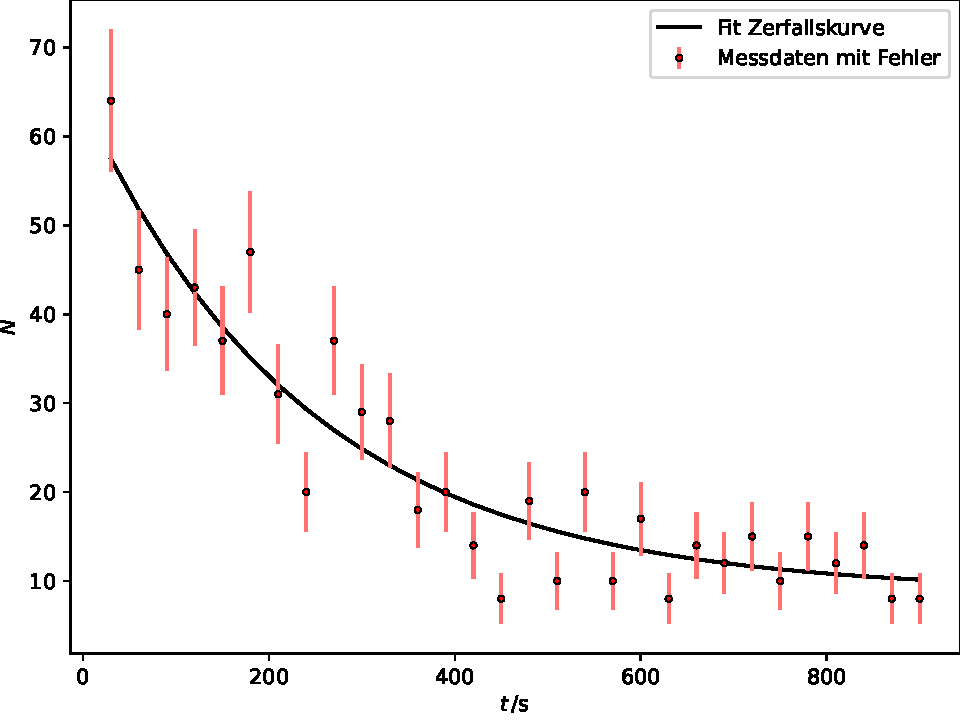
\includegraphics[width=\linewidth]{plots/vanadium_exp.pdf}
  \caption{Zerfallskurve von Vanadium.}
  \label{fig:vanadium_exp}
\end{figure}
Eine Funktion der Form 
\begin{equation*}
  g(x) = a\cdot exp(-b\cdot(x+c)) + d
\end{equation*}
wird an die Messdaten angepasst. Die Ausgleichsrechnung mit scipy \cite{scipy} ergibt die Parameter
\begin{align*}
  a &= \SI{2.29439086e-01}{}\\
  b &= \SI{4.10385420(0.82348965)e-03}{\frac{1}{s}}\\
  c &= \SI{-1.33547329e+03}{s}\\
  d &= \SI{8.77272198(2.83032112)}{}.\\
\end{align*}

Für den halblogarithmischen Plot in \autoref{fig:vanadium} werden die Werte aus \autoref{tab:vanadium2} verwendet. Da beim logarithmieren die Messdaten und Fehler zusammengestaucht werden,
wird aus übersichtlichen Gründen auf die Fehler verzichtet. 

\begin{figure}[H]
  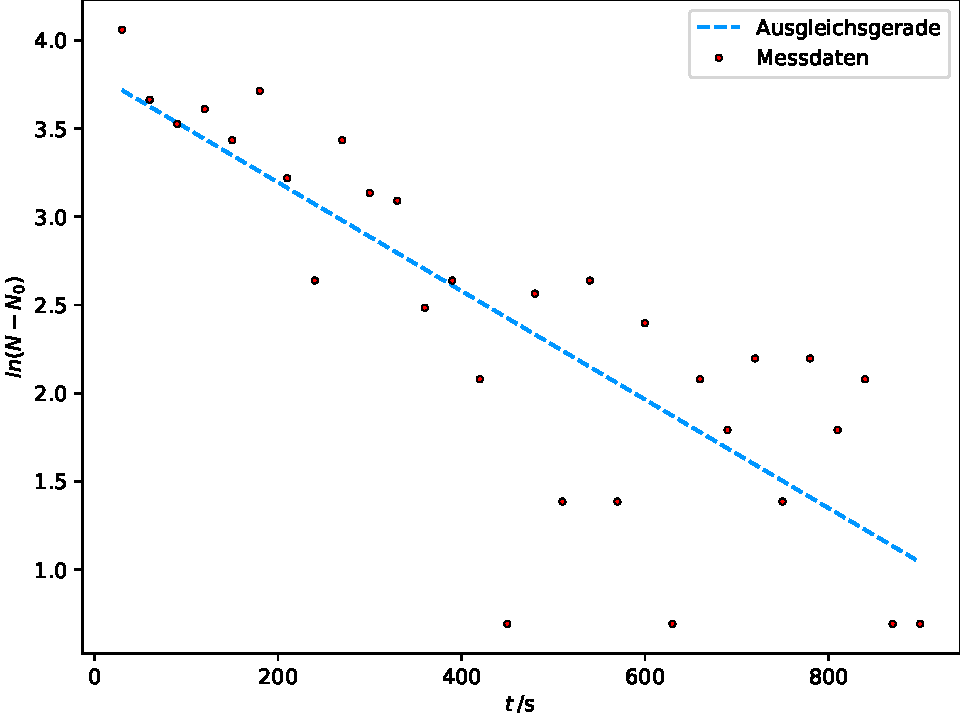
\includegraphics[width=\linewidth]{plots/vanadium.pdf}
  \caption{Halblogarithmischer Plot von Vanadium zur Bestimmung der Halbwertszeit.}
  \label{fig:vanadium}
\end{figure}

An die Messwerte wird eine lineare Funktion der Form
\begin{equation*}
  ln(N-N_0) = a\cdot x + b
\end{equation*}
gefitted. Die Parameter ergeben sich zu 
\begin{align*}
  a &= \SI{-3.07560534(0.4)e-03}{\frac{1}{s}}\\
  b &= \SI{3.81018748(0.21890378)}{}.\\
\end{align*}

Mit \autoref{eq:Halbwertszeit} folgt 
\begin{equation*}
  T = \frac{ln(2)}{|a|} = \SI{225(30)}{s}.
\end{equation*}

\subsection{Zerfall von Silber}
Für Silber wurden zwei Messreihen aufgenommen, um Ungenauigkeiten zu Beginn der Messung
zu minimieren. Die Messdaten sind in \autoref{tab:silber} aufgelistet.

\begin{table}[H]
  \centering
  \caption{Messergebnisse für die Vanadiumprobe}
  \resizebox{0.7\textwidth}{!}{
  \begin{tabular}{S[table-format=3] S[table-format=2(2)]}
      \toprule
      {$t\,/\symup{s}$} & {$N$} \\
      \midrule
      10  & 96 \\
      20  & 103 \\
      20  & 67 \\
      40  & 60 \\
      50  & 45 \\
      60  & 24 \\
      70  & 22 \\
      80  & 30 \\
      90  & 32 \\
      100 & 22 \\
      110 & 22 \\
      120 & 25 \\
      130 & 24 \\
      140 & 18 \\
      150 & 21 \\
      160 & 8 \\
      170 & 11 \\
      180 & 10 \\
      190 & 15 \\
      200 & 10 \\
      210 & 7 \\
      220 & 13 \\
      \bottomrule
  \end{tabular}
  \begin{tabular}{S[table-format=3] S[table-format=2(2)]}
      \toprule
      {$t\,/\symup{s}$} & {$N$} \\
      \midrule
      230 & 9\\
      240 & 9\\
      250 & 15\\
      260 & 11\\
      270 & 7\\
      280 & 9\\
      290 & 17\\
      300 & 5\\
      310 & 10\\
      320 & 6\\
      330 & 5\\
      340 & 10\\
      350 & 8\\
      360 & 9\\
      370 & 6\\
      380 & 6\\
      390 & 10\\
      400 & 4\\
      410 & 3\\
      420 & 5\\
      430 & 3\\
          &         \\
      \bottomrule
  \end{tabular}
  \begin{tabular}{S[table-format=3] S[table-format=2(2)]}
    \toprule
    {$t\,/\symup{s}$} & {$N$} \\
    \midrule
    10  & 123 \\
    20  & 105 \\
    20  & 91 \\
    40  & 80 \\
    50  & 57 \\
    60  & 43 \\
    70  & 42 \\
    80  & 40 \\
    90  & 28 \\
    100 & 26 \\
    110 & 14 \\
    120 & 22 \\
    130 & 18 \\
    140 & 19 \\
    150 & 15 \\
    160 & 14 \\
    170 & 10 \\
    180 & 9 \\
    190 & 17 \\
    200 & 7 \\
    210 & 7 \\
    220 & 18 \\
    \bottomrule
\end{tabular}
\begin{tabular}{S[table-format=3] S[table-format=2(2)]}
    \toprule
    {$t\,/\symup{s}$} & {$N$} \\
    \midrule
    230 & 8\\
    240 & 11\\
    250 & 11\\
    260 & 10\\
    270 & 7\\
    280 & 6\\
    290 & 6\\
    300 & 8\\
    310 & 13\\
    320 & 7\\
    330 & 9\\
    340 & 6\\
    350 & 8\\
    360 & 5\\
    370 & 4\\
    380 & 4\\
    390 & 5\\
    400 & 5\\
    410 & 5\\
    420 & 4\\
    430 & 7\\
        &         \\
    \bottomrule
\end{tabular}
  }
  \label{tab:silber}
\end{table}

Die Auswertung wird für beide Messreihen durchgeführt. Wie bei dem Zerfall von Vanadium werden bei den Zerfallskurven die unbereinigten Messwerte genommen, um einen 
Vergleichswert für den Nulleffekt zu errechnen. In \autoref{fig:silber1exp} und \autoref{fig:silber2exp} ist die Zeit $t$ gegen die Impulse $N$ mit Fehler $\sqrt(N)$ aufgetragen.
\begin{figure}[H]
  \centering
  \begin{subfigure}[b]{0.49\textwidth}
      \centering
      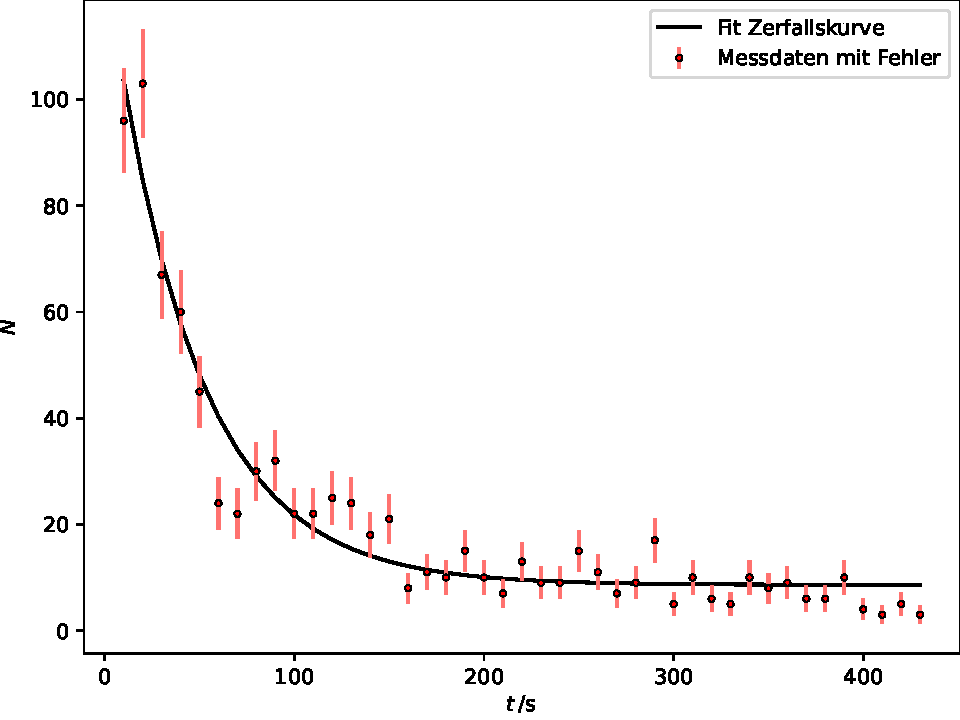
\includegraphics[width=7.5cm, height=6cm]{plots/messung1_silber_expfit.pdf}
      \caption[]
      {{\small Messreihe 1 Zerfallskurve.}}    
      \label{fig:silber1exp}
  \end{subfigure}
  \hfill
  \begin{subfigure}[b]{0.49\textwidth}  
      \centering 
      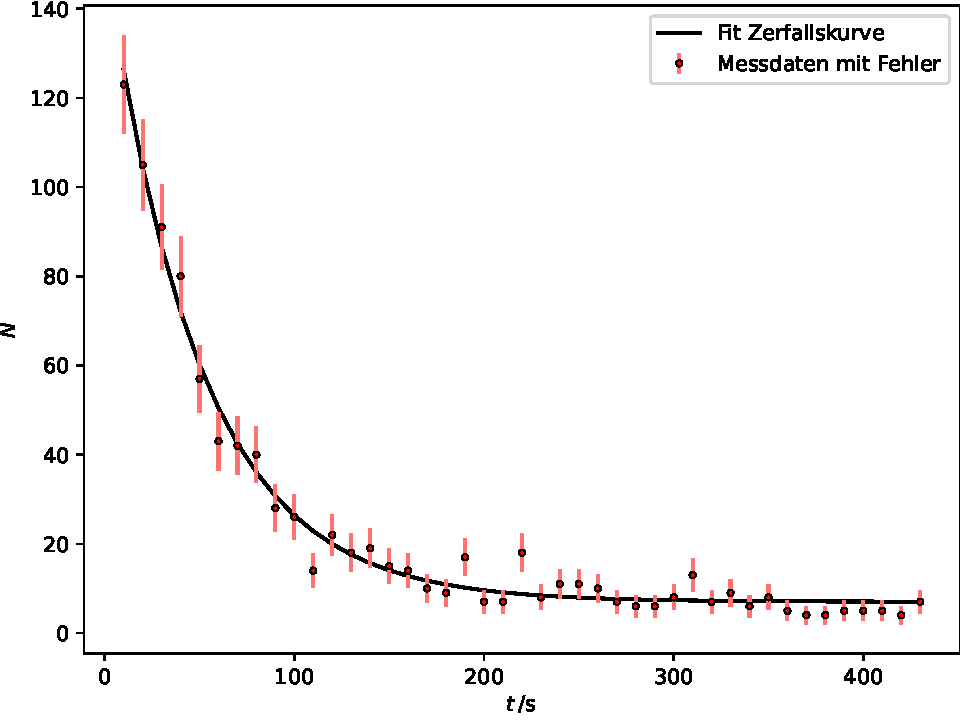
\includegraphics[width=7.5cm, height=6cm]{plots/messung2_silber_expfit.pdf}
      \caption[]
      {{\small Messreihe 2 Zerfallskurve.}}    
      \label{fig:silber2exp}
  \end{subfigure}
\end{figure}

Für beide Messreihen wird eine Funktion der Form
\begin{equation*}
  g(x) = a\cdot exp(-b\cdot(x+c)) + d
\end{equation*}
an die Messdaten angepasst. Die Ausgleichsrechnung mit scipy \cite{scipy} ergibt die Parameter
\begin{align*}
  a_1 &= \SI{2.22277337e-01}{}\\
  b_1 &= \SI{2.19599057(0.1)e-02}{\frac{1}{s}}\\
  c_1 &= \SI{-2.85837744e+02}{s}\\
  d_1 &= \SI{8.61292360(1.20099332)}{}\\
\end{align*}
und 
\begin{align*}
  a_2 &= \SI{1.99837584e-01}{}\\
  b_2 &= \SI{2.01934044(0.08)e-02}{\frac{1}{s}}\\
  c_2 &= \SI{-3.26517541e+02}{s}\\
  d_2 &= \SI{7.02044544(0.7723001)}{}.\\
\end{align*}
In einem halblogarithmischen Plot können die gleichzeitig auftretenden Zerfälle in einen langlebigen und kurzlebigen Zerfall aufgeteilt werden.
Hierfür werden die bereinigten Impulse $ln(N-N_0)$ und die Zeit $t$ eingetragen. Auf die Fehler wird in dieser Darstellung wieder verzichtet.
\begin{figure}[H]
  \centering
  \begin{subfigure}[b]{0.49\textwidth}
      \centering
      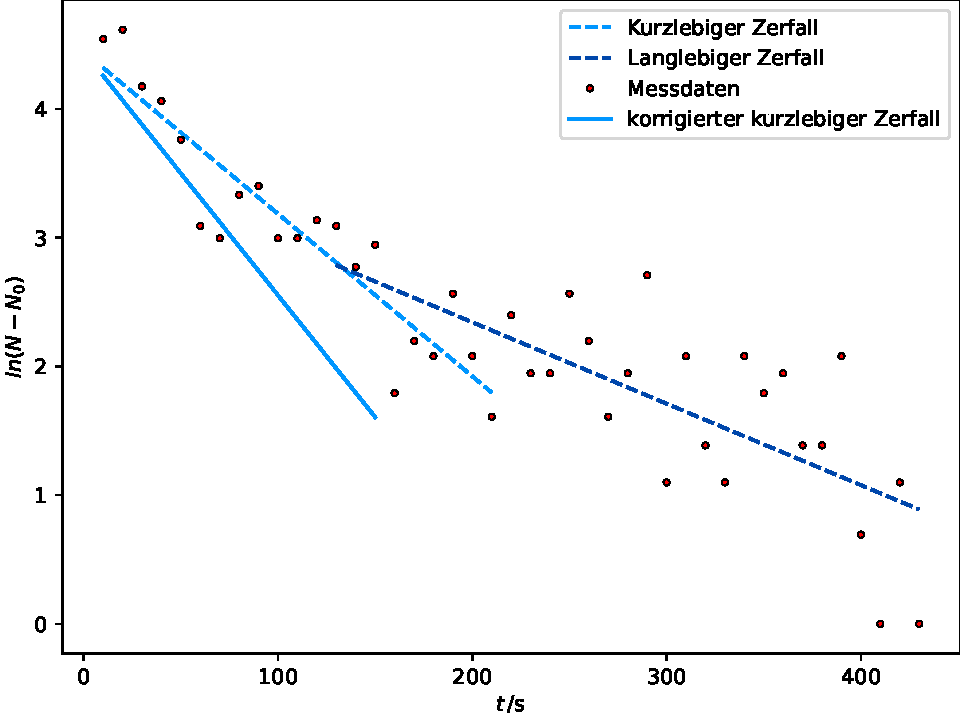
\includegraphics[width=7.5cm, height=6cm]{plots/messung1_silber.pdf}
      \caption[]
      {{\small Messreihe 1 halblogarithmische Darstellung.}}    
      \label{fig:silber1exp}
  \end{subfigure}
  \hfill
  \begin{subfigure}[b]{0.49\textwidth}  
      \centering 
      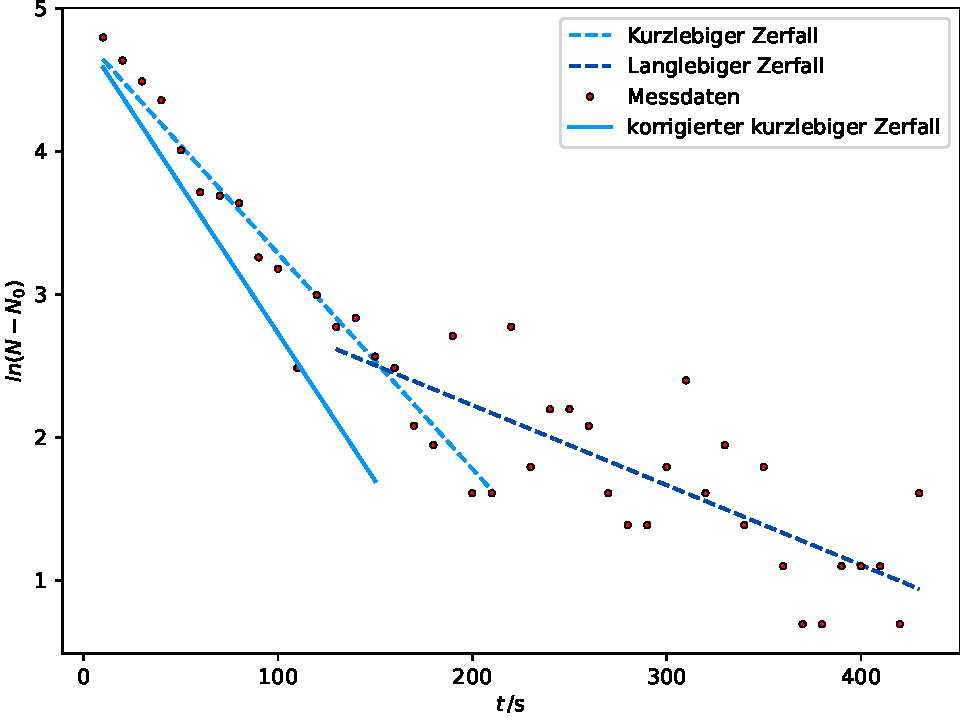
\includegraphics[width=7.5cm, height=6cm]{plots/messung2_silber.pdf}
      \caption[]
      {{\small Messreihe 2 halblogarithmische Darstellung.}}    
      \label{fig:silber2exp}
  \end{subfigure}
\end{figure}

Es wird hier jeweils ein Zeitpunkt $t*$ festgelegt, bei dem der kurzlebige Zerfall keinen großen Beitrag zum Gesamtzerfall leistet. Vor und nach diesem Zeitpunkt wird 
eine Ausgleichsgerade durch die Messpunkte gelegt. Die berechneten Parameter sind
\begin{align*}
  a_{1a} &= \SI{-0.0126165(0.00117734)}{\frac{1}{s}}\\
  a_{1b} &= \SI{-0.00632436(0.00091404)}{\frac{1}{s}}\\
  b_{1a} &= \SI{4.44647688(0.14783285)}{}\\
  b_{1b} &= \SI{3.60759803(0.26168668)}{}\\
\end{align*}
und 
\begin{align*}
  a_{1a} &= \SI{-0.01506289(0.0009466)}{\frac{1}{s}}\\
  a_{1b} &= \SI{-0.00558562(0.0007023)}{\frac{1}{s}}\\
  b_{1a} &= \SI{4.79253545(0.11886046)}{}\\
  b_{1b} &= \SI{3.34191341(0.20106708)}{}\\
\end{align*}
Hierbei steht der Index $1a$ für die Steigung der Geraden im Bereich vor $t*$ von Messreihe 1, der Index $1b$ für die Steigung der Geraden im Bereich nach $t*$ von Messreihe 1
usw.\\
Um nun den kurzlebigen und langlebigen Zerfall zu trennen, wird näherungsweise davon ausgegangen, dass ab dem Zeitpunkt $t*$ größtenteils nur noch der langlebige Zerfall 
stattfindet. Um den kurzlebigen Zerfall zu erhalten, muss wird die Steigung des langlebigen Zerfalls von der Gesamtsteigung in Bereich (a) abgezogen. Es gilt also 
\begin{equation*}
  a_{neu} = a_{a} - a_{b}.
\end{equation*}
Die korrigierten kurzlebigen Zerfälle sind ebenfalls in \autoref{fig:silber1exp} bzw. \autoref{fig:silber2exp} eingezeichnet.
Mit den ausgewerteten Daten lässt sich nun die jeweilige Halbwertszeit bestimmen.
Für die erste Messreihe ergibt sich mit \autoref{eq:}
\begin{equation*}
  T_{kurz_{1}} = \SI{37(4)}{s} \text{ und } T_{lang_{1}} = \SI{110(16)}{s} 
\end{equation*}
und für die zweite
\begin{equation*}
  T_{kurz_{2}} = \SI{33.6(2.7)}{s} \text{ und } T_{lang_{2}} = \SI{124(16)}{s}.
\end{equation*}
